\documentclass[bigtut]{tutorial}\usepackage[]{graphicx}\usepackage[]{color}
%% maxwidth is the original width if it is less than linewidth
%% otherwise use linewidth (to make sure the graphics do not exceed the margin)
\makeatletter
\def\maxwidth{ %
  \ifdim\Gin@nat@width>\linewidth
    \linewidth
  \else
    \Gin@nat@width
  \fi
}
\makeatother

\definecolor{fgcolor}{rgb}{0.345, 0.345, 0.345}
\newcommand{\hlnum}[1]{\textcolor[rgb]{0.686,0.059,0.569}{#1}}%
\newcommand{\hlstr}[1]{\textcolor[rgb]{0.192,0.494,0.8}{#1}}%
\newcommand{\hlcom}[1]{\textcolor[rgb]{0.678,0.584,0.686}{\textit{#1}}}%
\newcommand{\hlopt}[1]{\textcolor[rgb]{0,0,0}{#1}}%
\newcommand{\hlstd}[1]{\textcolor[rgb]{0.345,0.345,0.345}{#1}}%
\newcommand{\hlkwa}[1]{\textcolor[rgb]{0.161,0.373,0.58}{\textbf{#1}}}%
\newcommand{\hlkwb}[1]{\textcolor[rgb]{0.69,0.353,0.396}{#1}}%
\newcommand{\hlkwc}[1]{\textcolor[rgb]{0.333,0.667,0.333}{#1}}%
\newcommand{\hlkwd}[1]{\textcolor[rgb]{0.737,0.353,0.396}{\textbf{#1}}}%

\usepackage{framed}
\makeatletter
\newenvironment{kframe}{%
 \def\at@end@of@kframe{}%
 \ifinner\ifhmode%
  \def\at@end@of@kframe{\end{minipage}}%
  \begin{minipage}{\columnwidth}%
 \fi\fi%
 \def\FrameCommand##1{\hskip\@totalleftmargin \hskip-\fboxsep
 \colorbox{shadecolor}{##1}\hskip-\fboxsep
     % There is no \\@totalrightmargin, so:
     \hskip-\linewidth \hskip-\@totalleftmargin \hskip\columnwidth}%
 \MakeFramed {\advance\hsize-\width
   \@totalleftmargin\z@ \linewidth\hsize
   \@setminipage}}%
 {\par\unskip\endMakeFramed%
 \at@end@of@kframe}
\makeatother

\definecolor{shadecolor}{rgb}{.97, .97, .97}
\definecolor{messagecolor}{rgb}{0, 0, 0}
\definecolor{warningcolor}{rgb}{1, 0, 1}
\definecolor{errorcolor}{rgb}{1, 0, 0}
\newenvironment{knitrout}{}{} % an empty environment to be redefined in TeX

\usepackage{alltt}
\unitcode{MATH1005}
        \unitname{Statistics}
        \semester{Summer/Winter/Semester2}
        \sheetnumber5

\usepackage{graphicx}
\usepackage{hyperref}
%\withsolutions
\IfFileExists{upquote.sty}{\usepackage{upquote}}{}
\begin{document}
\lettersfirst

\begin{tutorial}

%\begin{displaybox}
%This tutorial explores probability. \\
%Most of the questions involve hand calculations, not R.  \\
%There are lots of questions, so work carefully through some questions in your tutorial \\
%and complete the rest at home. \\
%The 1st 20 minutes of class will be Online Quiz 1.\\
%\end{displaybox}

\begin{center}
\begin{tabular}{| ll |} \hline
& \\
{\bf Probability} &  \\
For 2 events $A$ and $B$ on the same sample space $\Omega$  & \\
$A$ and $B$ are mutually exclusive &   $P(A \cap B) = 0$    \\
$A$ and $B$ are independent & $P(A \cap B) = P(A) P(B)$      \\ 
the union of $A$ and $B$  & $P(A \cup B) = P(A) +  P(B) - P(A \cap B)$   \\
probability of $A$ conditional on $B$  & $P(A|B) = \frac{ P(A \cap B) }{ P(B) } $ \\ 
& \\  \hline
\end{tabular}
\end{center}

\begin{center}
\begin{tabular}{| ll |} \hline
& \\
{\bf Random Variables} &  \\
For a random variable $X$ on the sample space $\Omega$ & \\
Probability Distribution (Discrete) & $\{ x, P(X=x) \}$     \\
Cumulative Distribution Function (CDF) &   $F(x) = P(X \leq x)$    \\ \hline
\end{tabular}
\end{center}


\begin{questions}
\vspace{.5cm}
\question Simulating `Fair' Coin Tosses \\
Using classical probability, we say that a fair coin has $P(\mbox{Head}) = P(\mbox{Tail}) = 0.5$.  
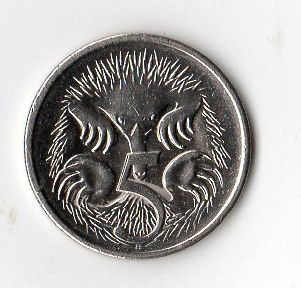
\includegraphics[height=1cm]{5c.jpg} \\

\begin{parts}
\part Estimate $P(\mbox{Head})$ and $P(\mbox{Tail})$  using the following simulation of 10 tosses.

\begin{knitrout}
\definecolor{shadecolor}{rgb}{0.969, 0.969, 0.969}\color{fgcolor}\begin{kframe}
\begin{alltt}
\hlstd{x}\hlkwb{=}\hlkwd{c}\hlstd{(}\hlstr{"H"}\hlstd{,}\hlstr{"T"}\hlstd{)}
\hlstd{toss}\hlkwb{=}\hlkwd{sample}\hlstd{(x,}\hlnum{10}\hlstd{,}\hlkwc{replace}\hlstd{=}\hlnum{TRUE}\hlstd{)}
\hlkwd{table}\hlstd{(toss)}
\end{alltt}
\end{kframe}
\end{knitrout}

Note: if you want to redo the same simulation, you can set a seed: Eg {\tt set.seed(1234)}

\vspace{.5cm}
\part Repeat using a simulation of size 10000.

\vspace{.5cm}
\part How do your results compare to John Kerrich? \\
{\tiny {https://en.wikipedia.org/wiki/John\_Edmund\_Kerrich}}
\end{parts}

\begin{solution}

(a) 
Each simulation will be different. \\

Example: 
\begin{knitrout}
\definecolor{shadecolor}{rgb}{0.969, 0.969, 0.969}\color{fgcolor}\begin{kframe}
\begin{alltt}
\hlkwd{set.seed}\hlstd{(}\hlnum{1234}\hlstd{)}
\hlstd{x}\hlkwb{=}\hlkwd{c}\hlstd{(}\hlstr{"H"}\hlstd{,}\hlstr{"T"}\hlstd{)}
\hlstd{toss}\hlkwb{=}\hlkwd{sample}\hlstd{(x,}\hlnum{10}\hlstd{,}\hlkwc{replace}\hlstd{=}\hlnum{TRUE}\hlstd{)}
\hlkwd{table}\hlstd{(toss)}
\end{alltt}
\begin{verbatim}
## toss
## H T 
## 3 7
\end{verbatim}
\end{kframe}
\end{knitrout}

$P(\mbox{Head}) = 0.7$. \\

(b) Example: 10000 tosses. 

\begin{knitrout}
\definecolor{shadecolor}{rgb}{0.969, 0.969, 0.969}\color{fgcolor}\begin{kframe}
\begin{alltt}
\hlkwd{set.seed}\hlstd{(}\hlnum{1234}\hlstd{)}
\hlstd{x}\hlkwb{=}\hlkwd{c}\hlstd{(}\hlnum{0}\hlstd{,}\hlnum{1}\hlstd{)}    \hlcom{#Let 1 represent a Head}
\hlstd{toss}\hlkwb{=}\hlkwd{sample}\hlstd{(x,}\hlnum{10000}\hlstd{,}\hlkwc{replace}\hlstd{=}\hlnum{TRUE}\hlstd{)}
\hlkwd{table}\hlstd{(toss)}
\end{alltt}
\begin{verbatim}
## toss
##    0    1 
## 4990 5010
\end{verbatim}
\end{kframe}
\end{knitrout}

$P(\mbox{Head}) = 0.5010$. \\

(c) Kerrich's result: $P(\mbox{Head}) = 0.5067$.
\end{solution}


\question Simulating an unfair die  \\

A six-sided die is loaded in such a way that every even number is twice as likely to
occur as every odd number.  The die is tossed once. \\

\begin{parts}

\part Fill out the following probability distribution. 

\begin{center}
\begin{tabular}{| l | l | l | l | l | l | l | l |} \hline
x & 1 \hspace{1cm}  & 2 \hspace{1cm} & 3 \hspace{1cm} & 4 \hspace{1cm} & 5 \hspace{1cm} & 6 \hspace{1cm} &  Total \\ \hline
P(X=x) && & & & & & 1 \\  \hline
\end{tabular}
\end{center}

\vspace{.5cm}
\part What is the probability that a number (strictly) less than 4 occurs? 

\vspace{.5cm}
\part  Let $A$ be the event that an even number occurs and let $B$ be the event that a number divisible by 3 occurs. Find $P(A \cap B)$ and $P(A \cup B)$.
 
\vspace{.5cm}
\part
Simulate (a) and (b).

\begin{knitrout}
\definecolor{shadecolor}{rgb}{0.969, 0.969, 0.969}\color{fgcolor}\begin{kframe}
\begin{alltt}
\hlstd{x}\hlkwb{=}\hlkwd{c}\hlstd{(}\hlnum{1}\hlstd{,}\hlnum{2}\hlstd{,}\hlnum{2}\hlstd{,}\hlnum{3}\hlstd{,}\hlnum{4}\hlstd{,}\hlnum{4}\hlstd{,}\hlnum{5}\hlstd{,}\hlnum{6}\hlstd{,}\hlnum{6}\hlstd{)}
\hlstd{toss}\hlkwb{=}\hlkwd{sample}\hlstd{(x,}\hlnum{10000}\hlstd{,}\hlkwc{replace}\hlstd{=}\hlnum{TRUE}\hlstd{)}
\hlkwd{table}\hlstd{(toss)}
\end{alltt}
\end{kframe}
\end{knitrout}
\end{parts}



\begin{solution}

(a) \\
\begin{tabular}{| l | l | l | l | l | l | l | l |} \hline
x & 1 \hspace{1cm}  & 2 \hspace{1cm} & 3 \hspace{1cm} & 4 \hspace{1cm} & 5 \hspace{1cm} & 6 \hspace{1cm} &  Total \\ \hline
P(X=x) & 1/9    & 2/9 & 1/9 & 2/9 & 1/9 & 2/9 & 1 \\  \hline
\end{tabular}

\vspace{.5cm}
Reasoning:
\\
For some value $p$, the weights for each outcome are as follows \\
\begin{tabular}{|l|c|c|c|c|c|c| c|}
\hline
x & 1 & 2 & 3 & 4 & 5 & 6 & Total \\\hline
P(X=x) & $p$ & $2p$ & $p$ & $2p$ & $p$ & $2p$ & 1 \\ \hline
\end{tabular}

\vspace{.5cm}
Since the weights must add to 1, $9p=1$, hence $p=1/9$.

\vspace{.5cm}
(b)
$P(\text{number strictly less than 4 occurs}) = P(1) +P(2)+P(3) = 4/9$.
  
\vspace{.5cm}           
(c)
 $A = \{ 2,4,6 \}$ and $B = \{ 3,6 \}$. \\
 $P(A \cup B) = P(\{ 2,3,4,6 \}) = 7/9$ \\
 $P(A \cap B) = P(\{ 6 \}) = 2/9$ \\              
\end{solution}



\vspace{.5cm}
\question Using Hospital Data to Estimate Probabilities \\

Hospital data of discharged patients contains the following columns:
\begin{verbatim}
   Column  Label
   1       ID no.           2       Duration of hospital stay
   3       Age              4       Sex  1=male  2=female
   5       First temperature following admission
   6       First WBC(x1000) following admission
   7       Received antibiotic 1=yes  2=no
   8       Received bacterial culture 1=yes  2=no
   9       Service 1=med 2=surg.
\end{verbatim}

\vspace{.5cm}
\begin{parts}
\part Upload the data and have a look at it.

\begin{knitrout}
\definecolor{shadecolor}{rgb}{0.969, 0.969, 0.969}\color{fgcolor}\begin{kframe}
\begin{alltt}
\hlstd{data}\hlkwb{=}\hlkwd{read.table}\hlstd{(}\hlkwc{file}\hlstd{=}\hlkwd{url}\hlstd{(}\hlstr{"http://www.maths.usyd.edu.au/u/UG/WS/WS1005/r/Hospital.txt"}\hlstd{),}
                \hlkwc{skip}\hlstd{=}\hlnum{1}\hlstd{)}
\end{alltt}
\end{kframe}
\end{knitrout}

\vspace{.5cm}
\part How many patients were discharged?

\begin{knitrout}
\definecolor{shadecolor}{rgb}{0.969, 0.969, 0.969}\color{fgcolor}\begin{kframe}
\begin{alltt}
\hlkwd{dim}\hlstd{(data)}
\end{alltt}
\end{kframe}
\end{knitrout}

\vspace{.5cm}
\part How many patients were female?

\begin{knitrout}
\definecolor{shadecolor}{rgb}{0.969, 0.969, 0.969}\color{fgcolor}\begin{kframe}
\begin{alltt}
\hlstd{gender} \hlkwb{=} \hlstd{data[,}\hlnum{4}\hlstd{]}                      \hlcom{#Selects column4}
\hlstd{female} \hlkwb{=} \hlkwd{length}\hlstd{(gender[gender}\hlopt{==}\hlnum{2}\hlstd{])}     \hlcom{#Counts Females}
\end{alltt}
\end{kframe}
\end{knitrout}

\vspace{.5cm}
\part Isolate the data on treatments A  (antibiotic) and B (bacterial culture).
\begin{knitrout}
\definecolor{shadecolor}{rgb}{0.969, 0.969, 0.969}\color{fgcolor}\begin{kframe}
\begin{alltt}
\hlstd{a} \hlkwb{=} \hlstd{data[,}\hlnum{7}\hlstd{]}
\hlstd{b} \hlkwb{=} \hlstd{data[,}\hlnum{8}\hlstd{]}
\end{alltt}
\end{kframe}
\end{knitrout}

\vspace{.5cm}
\part Count the number of patients receiving the treatments.
\begin{knitrout}
\definecolor{shadecolor}{rgb}{0.969, 0.969, 0.969}\color{fgcolor}\begin{kframe}
\begin{alltt}
\hlkwd{length}\hlstd{(a[a}\hlopt{==}\hlnum{1}\hlstd{])}             \hlcom{#Patients receiving A}
\hlkwd{length}\hlstd{(b[b}\hlopt{==}\hlnum{1}\hlstd{])}
\hlkwd{length}\hlstd{(a[a}\hlopt{==}\hlnum{1} \hlopt{&} \hlstd{b}\hlopt{==}\hlnum{1}\hlstd{])}      \hlcom{#Patients receiving both A and B}
\hlkwd{length}\hlstd{(a[a}\hlopt{==}\hlnum{1} \hlopt{&} \hlstd{gender}\hlopt{==}\hlnum{2}\hlstd{])} \hlcom{#Female Patients receiving A}
\end{alltt}
\end{kframe}
\end{knitrout}

\vspace{.5cm}
\part Use the data to estimate the following probabilities. 

\begin{center}
\begin{tabular}{|l|c|c|c|c|} \hline
Event & $A$ \hspace{1cm} & $B$ \hspace{1cm} & $A \cap B$ \hspace{1cm} & $A | Female$ \hspace{1cm} \\ \hline
Probability & & & & \\ \hline
\end{tabular}
\end{center}

\vspace{.5cm}
\part Are the events A and B mutually exclusive? Are the events A and B independent?

\end{parts}




\begin{solution}
(a) 
\begin{verbatim}
> data
   V1 V2 V3 V4   V5 V6 V7 V8 V9
1   1  5 30  2 99.0  8  2  2  1
2   2 10 73  2 98.0  5  2  1  1
...
25 25  4 41  2 98.0  5  2  2  1
\end{verbatim}

\vspace{.5cm}
(b) 
The number of discharged patients is 25.

\vspace{.5cm}
(c) 
The number of female patients is 14.

\vspace{.5cm}
(f) \\
\begin{tabular}{|l|c|c|c|c|} \hline
Event & $A$ \hspace{1cm} & $B$ \hspace{1cm} & $A \cap B$ \hspace{1cm} & $A | Female$ \hspace{1cm} \\ \hline
Probability & 7/25 = 0.28 & 6/25 = 0.24  & 2/25 = 0.08 & 2/14 $\approx$ 0.14 \\ \hline
\end{tabular}

\vspace{.5cm}
(g) \\
As $P( A \cap B) \neq 0$, events A and B are not mutually exclusive. \\
As $P(A \cap B) \neq P(A)P(B)$, events A and B are not independent.
\end{solution}




\newpage
\hspace{-1cm} {\bf Extra Questions}


\vspace{.5cm}
\question Distribution of Total of three dice  \\

Suppose three fair six-sided dice are rolled independently and the numbers on the 3 top faces are added together. 

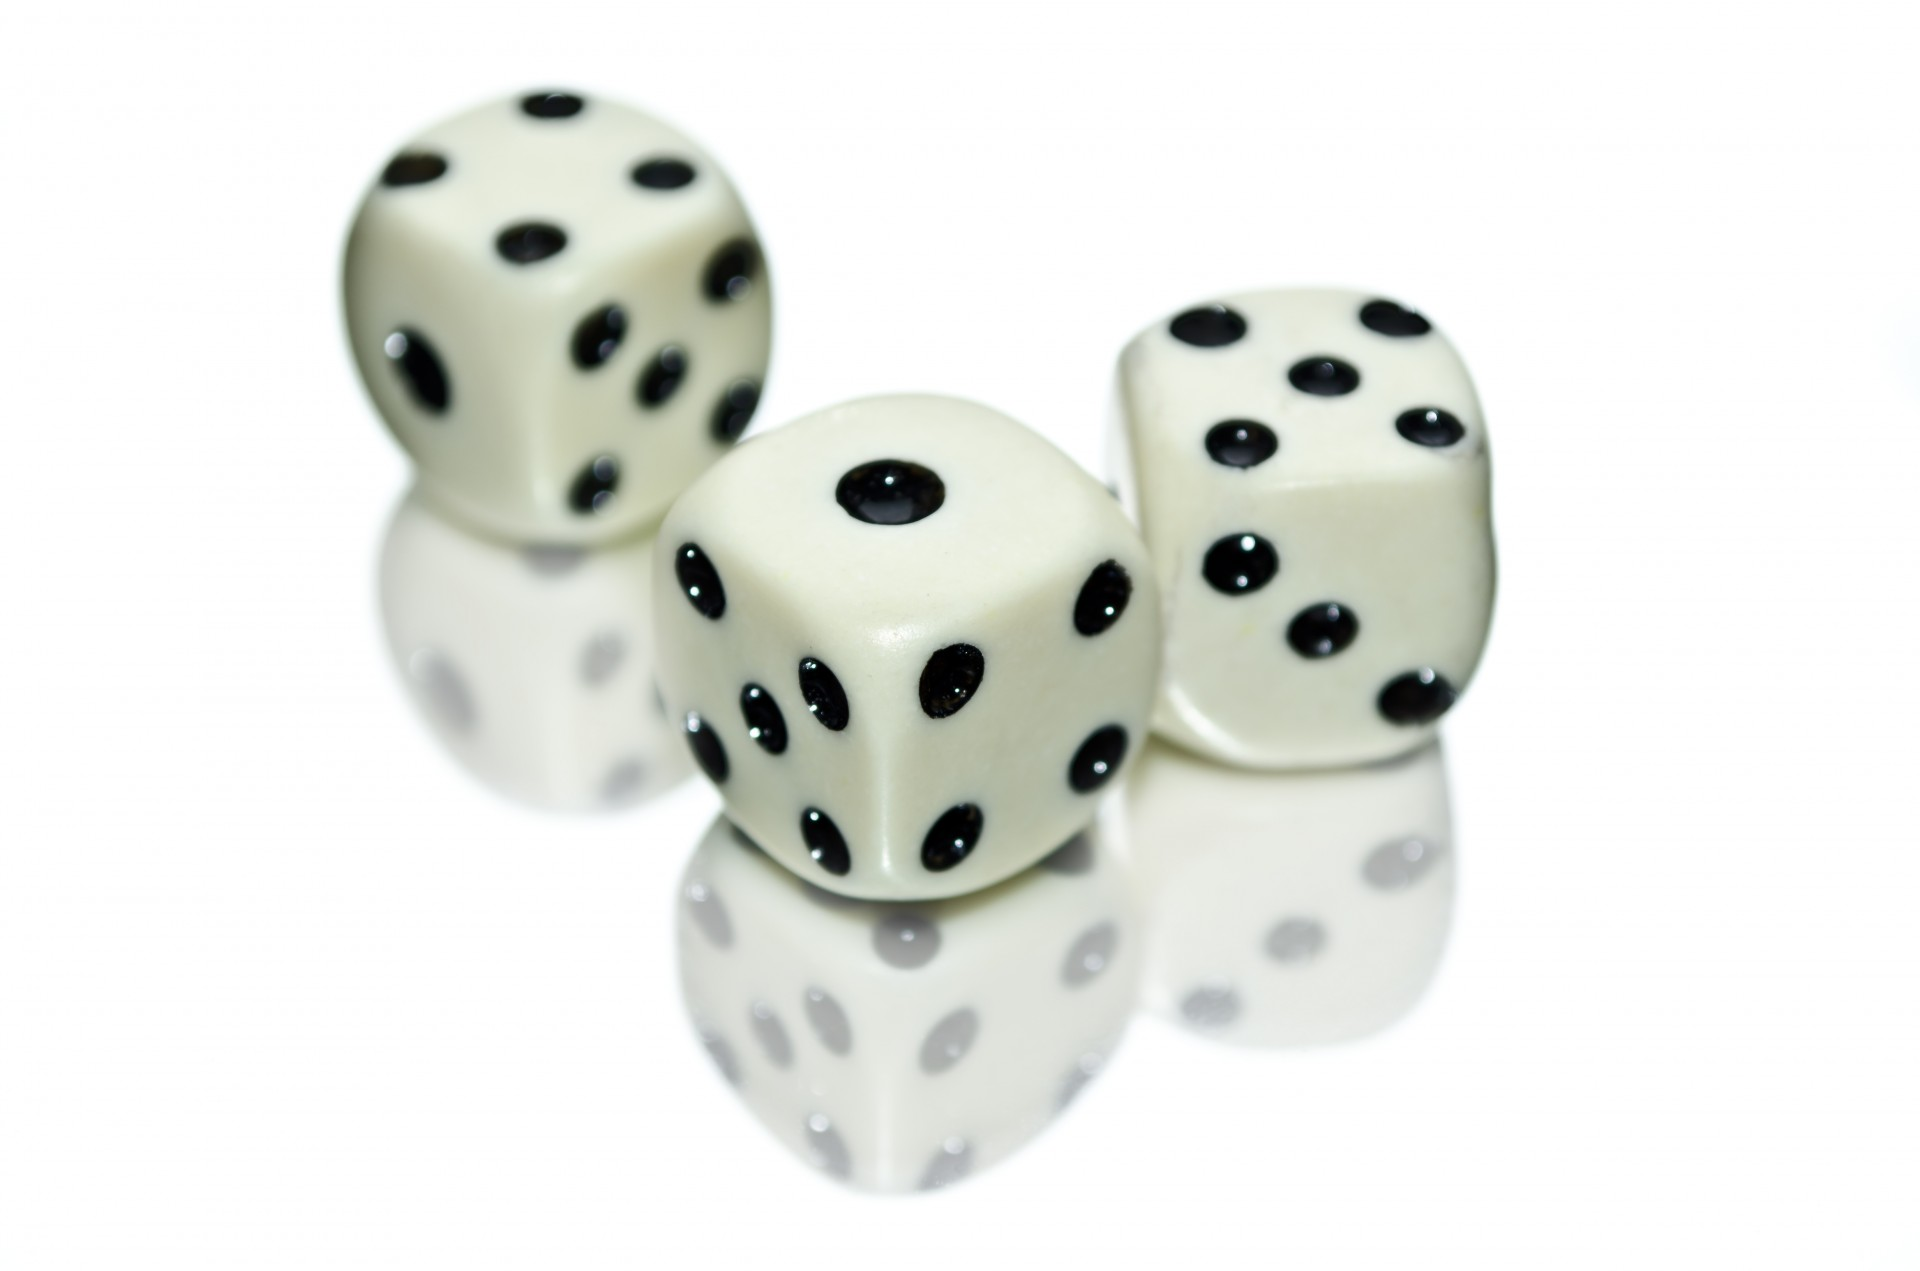
\includegraphics[height=1.4cm]{3Dice.jpg}

\begin{parts}
\part 
What is the total number of possible sequences  $\left\{1,1,1\right\}  \ldots \left\{6,6,6\right\}$?

\part
List the 3 sequences that give a  total of 4.

\part
What is the probability that the total is 4? 

\part
Estimate the probability using the following simulation.

\begin{knitrout}
\definecolor{shadecolor}{rgb}{0.969, 0.969, 0.969}\color{fgcolor}\begin{kframe}
\begin{alltt}
\hlstd{rolls} \hlkwb{=} \hlkwd{sample}\hlstd{(}\hlkwc{x}\hlstd{=}\hlkwd{c}\hlstd{(}\hlnum{1}\hlstd{,}\hlnum{2}\hlstd{,}\hlnum{3}\hlstd{,}\hlnum{4}\hlstd{,}\hlnum{5}\hlstd{,}\hlnum{6}\hlstd{),} \hlnum{3000}\hlstd{,}\hlkwc{replace}\hlstd{=T)} \hlcom{#Simulates 3000 random die rolls}
\hlstd{mat}\hlkwb{=}\hlkwd{matrix}\hlstd{(rolls,}\hlkwc{ncol}\hlstd{=}\hlnum{3}\hlstd{)} \hlcom{#Puts rolls into a 1000x3 matrix}
\hlstd{getsums}\hlkwb{=}\hlkwd{rowSums}\hlstd{(mat)} \hlcom{#Sums of each row}
\hlkwd{table}\hlstd{(getsums)} \hlcom{#Frequency table of the sums}
\end{alltt}
\end{kframe}
\end{knitrout}

Note: Each row of the matrix simulates a roll of the 3 dice. Hence, we have 1000 simulations.

\end{parts}

\begin{solution}
(a)
There are $6^3=216$ possible sequences, all equally likely. \\

(b)  112, 121, 211  \\

(c)
$P(\text{total is 4}) = 3/6^3 \approx 0.014$.

\vspace{.5cm}
(d)  Each simulation will be different. Using the following one:
\begin{verbatim}
getsums
  3   4   5   6   7   8   9  10  11  12  13  14  15  16  17  18 
  2  16  30  44  70  94 126 129 127 112 102  68  40  30   7   3 
\end{verbatim}
$P(\text{total is 4}) = 16/1000 \approx 0.016$.
\end{solution}




\question Two dependent events  \\

A smoke-detector system consists of two parts $A$ and $B$. If smoke occurs then $A$ detects
it with probability 0.95, $B$ detects it with probability
0.98 and both of them detect it with probability 0.94.  \\

\begin{parts}  

\part Write down $P(A), P(B)$ and $P(A \cap B)$.

\part Show that $A$ and $B$ are not independent.

\part What is the probability that the smoke will not be detected?

\part What is the probability that A will not detect the smoke, given that B did detect the smoke.

\part Extension: Estimate $P(A)$ and $P(B)$, using the total law of probability.

\begin{knitrout}
\definecolor{shadecolor}{rgb}{0.969, 0.969, 0.969}\color{fgcolor}\begin{kframe}
\begin{alltt}
\hlstd{outcome} \hlkwb{=} \hlkwd{c}\hlstd{(}\hlstr{"both detect"}\hlstd{,} \hlstr{"only A detects"}\hlstd{,} \hlstr{"only B detects"}\hlstd{,} \hlstr{"neither detects"}\hlstd{)}
\hlstd{probs} \hlkwb{=} \hlkwd{c}\hlstd{(}\hlnum{0.94}\hlstd{,} \hlnum{0.01}\hlstd{,} \hlnum{0.04}\hlstd{,} \hlnum{0.01}\hlstd{)}
\hlkwd{set.seed}\hlstd{(}\hlnum{1}\hlstd{)}
\hlstd{samp} \hlkwb{=} \hlkwd{sample}\hlstd{(outcome,} \hlnum{10000}\hlstd{, probs,} \hlkwc{replace} \hlstd{= T)}
\hlkwd{table}\hlstd{(samp)}
\end{alltt}
\end{kframe}
\end{knitrout}

\end{parts}


\begin{solution}
Let $A$ = detector A detects the smoke and $B$ = detector B detects the smoke. \\

(a) 
$P(A) = 0.95$, $P(B)=0.98$, $P(A \cap B)= 0.94$. \\

(b)
Check whether $P(A \cap B)=P(A)P(B)$. \\
$\text{LHS} = 0.94$. \\
$\text{RHS} = 0.95 \times 0.98=0.931$. \\
Hence, $A$ and $B$ are not independent. \\

(c)
$P(\text{smoke will not be detected}) = P(\text{neither A nor B works}) =  P(A' \cap B') = 1-P(A\cup B)$. \\
We have $P(A\cup B) = P(A)+P(B)-P(A\cap B) = 0.95+0.98-0.94 = 0.99$. \\
Hence, $P(\text{neither A nor B works}) = 1- 0.99 = 0.01$. 

\vspace{.5cm}
(d)
This is conditional probability. \\
$P(\text{A will not detect smoke}| \text{B did detect smoke}) 
= P(A' | B)
= \frac{ P(A' \cap B) }{ P(B)} = \frac{0.04}{0.98} \approx  0.0408$
where
$P(A'\cap B) = P(B)-P(A\cap B) = 0.98-0.94 = 0.04$.

\vspace{.5cm}
Note: Drawing a Venn diagram can assist in the working.

\vspace{.5cm}
(e)
\begin{knitrout}
\definecolor{shadecolor}{rgb}{0.969, 0.969, 0.969}\color{fgcolor}\begin{kframe}
\begin{verbatim}
## samp
##     both detect neither detects  only A detects  only B detects 
##            9367             103              96             434
\end{verbatim}
\end{kframe}
\end{knitrout}

$P(A) = \frac{9367}{10000} +  \frac{96}{10000} = 0.9463$. \\

$P(B) = \frac{9367}{10000} +  \frac{434}{10000} = 0.9801$. \\

\end{solution}


\question Three independent events \\

 Three football players will
attempt to kick a field goal. Let $A_1,A_2,A_3$ denote the events
that the field goal is made by player $1,2,3$, respectively. Assume
that $A_1$, $A_2$, $A_3$ are independent with $P(A_1)=0.5$,
$P(A_2)=0.7$ and $P(A_3)=0.6$. Compute the probability that exactly one
player is successful.


\begin{solution}
$P(\text{Exactly one person kicks a goal}) 
= P(A_1 \cap A_2^c \cap A_3^c) + P(A_1^c \cap A_2 \cap A_3^c) + P(A_1^c \cap A_2^c \cap A_3)$ \\

Using independence, \\
$P(\text{Exactly one person kicks a goal}) \\
= (0.5)(0.3)(0.4) + (0.5)(0.7)(0.4) + (0.5)(0.3)(0.6) \\
= 0.06+0.14+0.09 \\
= 0.29$

\end{solution}

\question Table of frequencies \\

In 1988 the Physicians' Health Study Research Group released
the results of a five-year experiment based on 22,071 people
between the ages of 40 and 84. The purpose was to determine whether
taking aspirin reduces the risk of a heart attack. The people had
been randomly assigned to one of two treatment groups: one group
took aspirin, the other took the placebo (non drug). The following information was
obtained.
$$
\begin{array}{|cl|c|c|}\hline
&& \mbox{\rm people with heart attack} & \mbox{\rm  people without heart
attack}
 \\\hline \mbox{\rm Aspirin}& & 104 &
10,933\\\hline \mbox{\rm Placebo}&  & 189 & 10,845 \\\hline
\end{array}
$$

\vspace{.5cm}
One person is selected by chance.
\begin{parts}
\part Let $A$ be the event that the selected person
had a heart attack. Find $P(A)$.
\part Let $B$ be the event that the selected person
took aspirin. Find $P(B)$.
\part Find the
probability that the selected person had a heart attack given
that they were in the Aspirin group.
\part Are $A$ and $B$ independent?
\end{parts}



\begin{solution}
(a) \\ 
$P(A) = (104+189)/22071 = 293/22071 \approx 0.013 $ \\

\vspace{.5cm}
(b) \\
$P(B) = (104+10933)/22071 = 11037/22071 \approx 0.5$ \\

\vspace{.5cm}
(c) \\
$P(A | B) = \frac{ P(A \cap B )}{P(B)} = \frac{104/22071}{11037/22071} = 104/11037 \approx 0.009$ \\

\vspace{.5cm}
(d) \\
Check whether $P(A \cap B) = P(A)P(B)$. \\
$LHS = P(A \cap B)  = 104/22071 \approx 0.005$ \\
$RHS = P(A)P(B) = (293/22071)(11037/22071) \approx 0.007$ \\
Hence $A$ and $B$ are not independent.

\end{solution}


\question  Deck of cards  \\

A standard deck of cards consists of 52 different cards, with 13 cards of each of the 4 suits (hearts, diamonds, spades and clubs). 5 cards are taken out without replacement and placed face-down on a table. \\
\begin{parts}
\part What is the probability that all 5 cards belong to the suit of hearts?
\part What is the probability that all 5 cards belong to the same suit?
\part What is the probability that exactly 4 cards belong to the suit of hearts?
\part If 4 of the cards are turned face-up on the table, and are all hearts, what is the probability that the 5th card also belongs to the suit of hearts?
\end{parts}


\begin{solution}
(a)
This can be modelled by a hypergeometric distribution, with $N=52$, $N_{1} = 13$ (hearts) and $N_{2} = 39$ (non hearts). Draw 5 cards without replacement. \\
Hence $P( \text{5 cards are all hearts}) = \frac{ {13 \choose 5} {39 \choose 0} } { {52 \choose 5} } = \frac{ {13 \choose 5} }{ {52 \choose 5} } \doteq 0.0005$.

\vspace{.5cm}
(b)
$P($5 cards same suit$) = P($5 cards hearts$) + P($5 cards clubs$) + P($5 cards diamonds$) + P($5 cards spades$) = 4 \times \frac{{13 \choose 5}{39 \choose 0}}{{52 \choose 5}} = 0.0019$

\vspace{.5cm}
(c)
$P(\text{4 cards are hearts, 1 card is non heart}) =
\frac{ {13 \choose 4} {39 \choose 1} }{{52 \choose 5}} \doteq 0.0107$

\vspace{.5cm}
(d)
If we know that 4 hearts are on the table, then of the 48 remaining cards, only 9 of them are hearts. Thus $P(\text{5th card is hearts, given first four are hearts} ) = \frac{ {9 \choose 1}{39 \choose 0} }{{48 \choose 1}} =\frac{9}{48} = 0.1875$.\\

Note: This can also be calculated using the conditional probability formula. Let A be the event for which the 5th card is hearts, and B the event in which 4 first cards are hearts. Thus
\begin{eqnarray*}
P(A|B) &=&  \frac{P(A \cap B)}{P(B) } \\
& = & \frac{ P(\text{first 5 cards are all hearts} ) }{            P(\text{first 4 cards are all hearts}) } \\
&=&  \frac{(a)}{ \frac{ {13 \choose 4}{39 \choose 0} }{{52 \choose 4} } } \\
& = & \frac{ \frac{ {13 \choose 5} }{ {52 \choose 5} }  }{ \frac{ {13 \choose 4} }{{52 \choose 4} } } \\   
 &=& 0.1875
\end{eqnarray*}

\end{solution}










\question  Probability with 3 tosses of a coloured die \\

A six-sided die has two of its faces white, one red and three green.  It is thrown three times in such a way that  each face is equally likely to land facing upwards and that each throw is independent.
Compute the probability that \\

  \begin{parts}
 \part
a white face is uppermost at each throw

\part
 the same colour is uppermost at each throw. 
 \end{parts}



\begin{solution}
(a) \\
Let $W_{i}$ be the event that White is uppermost on throw i. $i=1,2,3$. \\
Let $R_{i}$ be the event that Red is uppermost on throw i. $i=1,2,3$. \\
Let $G_{i}$ be the event that Green is uppermost on throw i. $i=1,2,3$. \\
 
If each of the 6 faces is equally likely, then $P(\text{White uppermost on throw i}) = P(W_i) = 2/6 = 1/3$, for $i=1,2,3$. \\ 
Similarly, $P(\text{Red uppermost on throw i}) = P(R_i) = 1/6$ \\ 
and $P(\text{Green uppermost on throw i}) = P(G_i) = 3/6 = 1/2$. \\ 
 
Using independence,\\
$P(\text{a white face is uppermost at each throw}) = P(W_{1})P(W_{2})P(W_{3}) = (1/3)^3 = 1/27$. \\

\vspace{.5cm}
(b)
$P(\text{the same colour is uppermost at each throw}) =  (1/3)^3 + (1/6)^3 + (1/2)^3 = 1/6$. \\

Reasoning: \\
$P(\text{the same colour is uppermost at each throw}) = P(\text{all red OR all white OR all green}) \\
= P\{(W_1\cap W_2\cap W_3) \cup (R_1\cap R_2\cap R_3) \cup (G_1\cap G_2\cap G_3) \}$ \\

As we have decomposed the event into three mutually exclusive events, it follows that \\
$P(\text{all the same colour})
= P(W_1\cap W_2\cap W_3) + P(R_1\cap R_2\cap R_3) + P(G_1\cap G_2\cap G_3)$. \\

As $W_{i}$, $R_{i}$ and $G_{i}$ are all independent, it follows that \\
$P(\text{all the same colour})
= P(W_1)P(W_2)P(W_3) + P(R_1)P(R_2)P(R_3) + P(G_1)P(G_2)P(G_3) = \\
 (1/3)^3 + (1/6)^3 + (1/2)^3$.

\end{solution}

\end{questions}
\end{tutorial}
\end{document}


\question Total of three dice \\

Suppose three fair six-sided dice are rolled independently and the numbers on the 3 top faces are added together. \\
 
\begin{parts}
\part 
What is the total number of possible sequences  $\left\{1,1,1\right\}  \ldots \left\{6,6,6\right\}$?

\part
How many different ways can the numbers $\left\{1,1,1\right\}$, $\left\{1,1,2\right\}$
, $\left\{1,1,3\right\}$, $\left\{1,2,2\right\}$, $\left\{1,1,4\right\}$, $\left\{1,2,3\right\}$, and $\left\{2,2,2\right\}$
can be arranged in order?

\part
What is the probability that the total is at most 6? 
\end{parts}

\begin{solution}
(a)
There are $6^3=216$ possible sequences, all equally likely.

\vspace{.5cm}
(b) \\
$\left\{1,1,1\right\}$ 1 way \\
$\left\{1,1,2\right\}$ 3 ways (i.e.\ 112, 121, 211) \\
$\left\{1,1,3\right\}$ 3 ways \\
$\left\{1,2,2\right\}$ 3 ways \\
$\left\{1,1,4\right\}$ 3 ways \\
$\left\{1,2,3\right\}$ 6 ways (i.e.\ 123, 132, 213, 231, 312, 321) \\
$\left\{2,2,2\right\}$ 1 way \\
Hence there is a total of 20 ways of getting a total at most 6.

\vspace{.5cm}
(c)
$P(\text{total is at most 6}) = 20/6^3 \approx 0.09$
\end{solution}





